\documentclass[aspectratio=169]{beamer}
\usepackage[utf8]{inputenc}
\usepackage{tikz}
\usepackage{graphicx}
\usepackage{xcolor}
\usepackage{fontspec}
\usepackage{listings}

\usetikzlibrary{shapes.geometric, arrows.meta, positioning, fit, calc}

% UofSC Colors
\definecolor{garnet}{HTML}{73000a}
\definecolor{darkgarnet}{HTML}{570008}
\definecolor{atlantic}{HTML}{466A9F}
\definecolor{congaree}{HTML}{1F414D}
\definecolor{horseshoe}{HTML}{65780B}
\definecolor{honeycomb}{HTML}{A49137}
\definecolor{gray90}{HTML}{363636}
\definecolor{gray70}{HTML}{5C5C5C}
\definecolor{gray50}{HTML}{A2A2A2}

% Beamer theme
\usetheme{default}
\usecolortheme{default}
\setbeamercolor{structure}{fg=garnet}
\setbeamercolor{title}{fg=white,bg=garnet}
\setbeamercolor{frametitle}{fg=white,bg=garnet}
\setbeamercolor{block title}{fg=white,bg=garnet}
\setbeamercolor{block body}{fg=black,bg=gray!10}
\setbeamercolor{item}{fg=garnet}
\setbeamercolor{normal text}{fg=black}
\setbeamertemplate{navigation symbols}{}
\setbeamertemplate{footline}[frame number]

% TikZ styles - sharp corners, straight lines
\tikzstyle{process} = [rectangle, minimum width=2.5cm, minimum height=0.8cm,
                       text centered, draw=black, fill=white, line width=0.5pt]
\tikzstyle{decision} = [rectangle, minimum width=2cm, minimum height=0.8cm,
                        text centered, draw=black, fill=garnet!20, line width=0.5pt]
\tikzstyle{io} = [rectangle, minimum width=2.5cm, minimum height=0.8cm,
                  text centered, draw=black, fill=atlantic!20, line width=0.5pt]
\tikzstyle{arrow} = [-{Stealth[length=2mm]}, line width=0.5pt]

\title{\textbf{VRIFA}}
\subtitle{VARTM Resin Infusion Flow-Front Assessment}
\author{Automated Flow-Front Detection for Composite Manufacturing}
\date{}

\begin{document}

%% SLIDE 1: INTRO
\begin{frame}
\titlepage
\begin{center}

\begin{tikzpicture}
\node[rectangle, draw=garnet, line width=1.5pt, minimum width=10cm, minimum height=1.2cm, fill=garnet!10] {
    \textcolor{garnet}{\textbf{Computer Vision for VARTM Process Monitoring}}
};
\end{tikzpicture}
\end{center}
\end{frame}

%% SLIDE 2: PROBLEM STATEMENT
\begin{frame}{The Challenge: VARTM Process Monitoring}
\begin{columns}[T]
\begin{column}{0.55\textwidth}
\textbf{Vacuum-Assisted Resin Transfer Molding (VARTM)}
\begin{itemize}
    \item Resin infuses dry fiber reinforcement under vacuum
    \item Flow front progression must be tracked
    \item Manual monitoring is labor-intensive
    \item Lighting variations cause false detections
\end{itemize}
\vspace{0.5cm}
\textbf{Key Insight:}
\begin{itemize}
    \item Dry fabric $\rightarrow$ \textbf{lighter} (reflects light)
    \item Wet fabric $\rightarrow$ \textbf{darker} (absorbs light)
\end{itemize}
\end{column}
\begin{column}{0.42\textwidth}
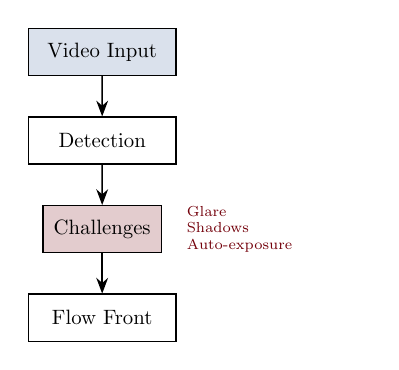
\begin{tikzpicture}[scale=0.75, transform shape]
    \node[io] (video) at (0,4) {Video Input};
    \node[process] (detect) at (0,2.5) {Detection};
    \node[decision] (challenge) at (0,1) {Challenges};
    \node[process] (output) at (0,-0.5) {Flow Front};

    \draw[arrow] (video) -- (detect);
    \draw[arrow] (detect) -- (challenge);
    \draw[arrow] (challenge) -- (output);

    \node[right=0.3cm of challenge, text width=3cm, font=\scriptsize] {
        \textcolor{garnet}{Glare}\\
        \textcolor{garnet}{Shadows}\\
        \textcolor{garnet}{Auto-exposure}
    };
\end{tikzpicture}
\end{column}
\end{columns}
\end{frame}

%% SLIDE 3: ALGORITHM PIPELINE
\begin{frame}{VRIFA Processing Pipeline}
\begin{center}
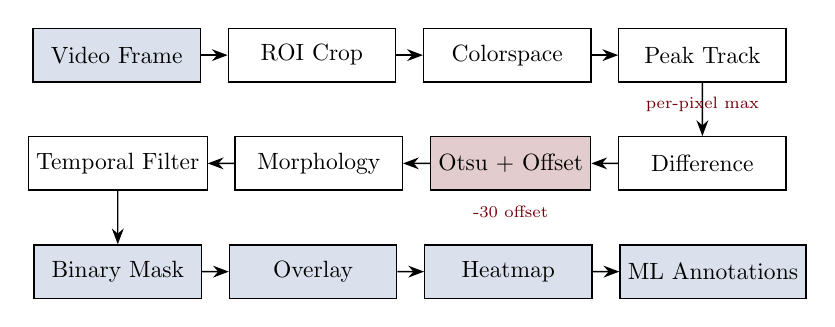
\begin{tikzpicture}[scale=0.85, transform shape, node distance=0.4cm]
    % Row 1
    \node[io] (input) {Video Frame};
    \node[process, right=of input] (roi) {ROI Crop};
    \node[process, right=of roi] (color) {Colorspace};
    \node[process, right=of color] (peak) {Peak Track};

    % Row 2
    \node[process, below=0.8cm of peak] (diff) {Difference};
    \node[decision, left=of diff] (thresh) {Otsu + Offset};
    \node[process, left=of thresh] (morph) {Morphology};
    \node[process, left=of morph] (temporal) {Temporal Filter};

    % Row 3
    \node[io, below=0.8cm of temporal] (mask) {Binary Mask};
    \node[io, right=of mask] (overlay) {Overlay};
    \node[io, right=of overlay] (heatmap) {Heatmap};
    \node[io, right=of heatmap] (annot) {ML Annotations};

    % Arrows Row 1
    \draw[arrow] (input) -- (roi);
    \draw[arrow] (roi) -- (color);
    \draw[arrow] (color) -- (peak);

    % Arrow down
    \draw[arrow] (peak) -- (diff);

    % Arrows Row 2
    \draw[arrow] (diff) -- (thresh);
    \draw[arrow] (thresh) -- (morph);
    \draw[arrow] (morph) -- (temporal);

    % Arrow down
    \draw[arrow] (temporal) -- (mask);

    % Arrows Row 3
    \draw[arrow] (mask) -- (overlay);
    \draw[arrow] (overlay) -- (heatmap);
    \draw[arrow] (heatmap) -- (annot);

    % Labels
    \node[below=0.1cm of peak, font=\scriptsize, text=garnet] {per-pixel max};
    \node[below=0.1cm of thresh, font=\scriptsize, text=garnet] {-30 offset};
\end{tikzpicture}
\end{center}
\end{frame}

%% SLIDE 4: KEY INNOVATION
\begin{frame}{Key Innovation: Darken-Only + Peak Reference}
\begin{columns}[T]
\begin{column}{0.48\textwidth}
\textbf{Darken-Only Detection}
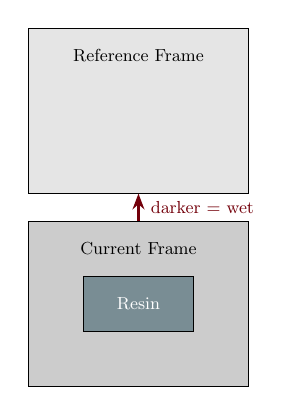
\begin{tikzpicture}[scale=0.7, transform shape]
    \draw[fill=gray!20, draw=black] (0,0) rectangle (4,3);
    \node at (2,2.5) {\small Reference Frame};

    \draw[fill=gray!40, draw=black] (0,-3.5) rectangle (4,-0.5);
    \node at (2,-1) {\small Current Frame};
    \draw[fill=congaree!60] (1,-2.5) rectangle (3,-1.5);
    \node[white] at (2,-2) {\small Resin};

    \draw[arrow, line width=1pt, garnet] (2,-0.5) -- (2,0);
    \node[right, garnet, font=\small] at (2.1,-0.25) {darker = wet};
\end{tikzpicture}
\vspace{0.3cm}

Only detects \textbf{darkening} pixels\\
Ignores: specular highlights, auto-exposure
\end{column}
\begin{column}{0.48\textwidth}
\textbf{Peak Brightness Reference}
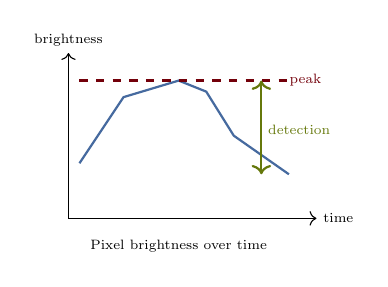
\begin{tikzpicture}[scale=0.7, transform shape]
    \draw[->] (0,0) -- (4.5,0) node[right] {\scriptsize time};
    \draw[->] (0,0) -- (0,3) node[above] {\scriptsize brightness};

    % Brightness curve
    \draw[thick, atlantic] (0.2,1) -- (1,2.2) -- (2,2.5) -- (2.5,2.3) -- (3,1.5) -- (4,0.8);

    % Peak line
    \draw[dashed, garnet, thick] (0.2,2.5) -- (4,2.5);
    \node[garnet, font=\scriptsize] at (4.3,2.5) {peak};

    % Detection zone
    \draw[<->, horseshoe, thick] (3.5,0.8) -- (3.5,2.5);
    \node[horseshoe, font=\scriptsize, right] at (3.5,1.6) {detection};

    \node[font=\scriptsize] at (2,-0.5) {Pixel brightness over time};
\end{tikzpicture}
\vspace{0.3cm}

Each pixel compared to its \textbf{historical maximum}\\
Handles: shadows, lighting stabilization
\end{column}
\end{columns}
\end{frame}

%% SLIDE 5: OUTPUTS
\begin{frame}{Multi-Format Outputs}
\begin{columns}[T]
\begin{column}{0.5\textwidth}
\textbf{Visualization Outputs}
\begin{itemize}
    \item \textbf{Binary Masks} -- raw detection
    \item \textbf{Overlays} -- red edge on original
    \item \textbf{Heatmaps} -- temporal accumulation
    \item \textbf{Videos} -- MP4 compilations
\end{itemize}

\vspace{0.5cm}
\textbf{ML Training Datasets}
\begin{itemize}
    \item \textcolor{garnet}{COCO} -- Detectron2, MMDetection
    \item \textcolor{atlantic}{YOLOv5/v8} -- Ultralytics
    \item \textcolor{congaree}{Darknet} -- YOLOv3/v4
\end{itemize}
\end{column}
\begin{column}{0.45\textwidth}
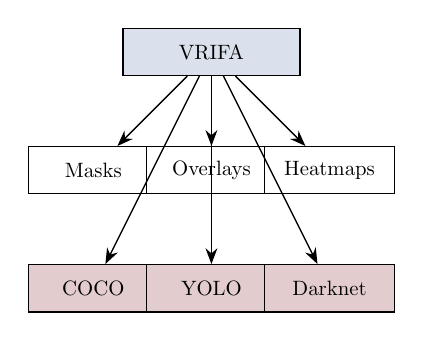
\begin{tikzpicture}[scale=0.75, transform shape]
    \node[io, minimum width=3cm] (vrifa) at (0,3) {VRIFA};

    \node[process, minimum width=2.2cm] (mask) at (-2,1) {Masks};
    \node[process, minimum width=2.2cm] (overlay) at (0,1) {Overlays};
    \node[process, minimum width=2.2cm] (heat) at (2,1) {Heatmaps};

    \node[decision, minimum width=2.2cm] (coco) at (-2,-1) {COCO};
    \node[decision, minimum width=2.2cm] (yolo) at (0,-1) {YOLO};
    \node[decision, minimum width=2.2cm] (dark) at (2,-1) {Darknet};

    \draw[arrow] (vrifa) -- (mask);
    \draw[arrow] (vrifa) -- (overlay);
    \draw[arrow] (vrifa) -- (heat);
    \draw[arrow] (vrifa) -- (coco);
    \draw[arrow] (vrifa) -- (yolo);
    \draw[arrow] (vrifa) -- (dark);
\end{tikzpicture}
\end{column}
\end{columns}
\end{frame}

%% SLIDE 6: DEMO
\begin{frame}{Demo: Processing Results}
\begin{columns}[T]
\begin{column}{0.48\textwidth}
\textbf{Input Frame}
\begin{center}

\includegraphics[width=0.9\textwidth]{output_input2_peak_annotated/formatCOCO/images/default/frame_000048.png}
\end{center}
\small Frame 48 -- Early infusion
\end{column}
\begin{column}{0.48\textwidth}
\textbf{Later Frame}
\begin{center}

\includegraphics[width=0.9\textwidth]{output_input2_peak_annotated/formatCOCO/images/default/frame_000088.png}
\end{center}
\small Frame 88 -- Advanced flow front
\end{column}
\end{columns}

\vspace{0.3cm}
\begin{center}
\texttt{python vrifa.py --video-path input.mp4 --write-videos}
\end{center}
\end{frame}

%% SLIDE 7: OUTRO
\begin{frame}
\begin{center}
\vspace{1cm}
{\Huge\textcolor{garnet}{\textbf{VRIFA}}}

\vspace{0.5cm}
{\Large VARTM Resin Infusion Flow-Front Assessment}

\vspace{1cm}
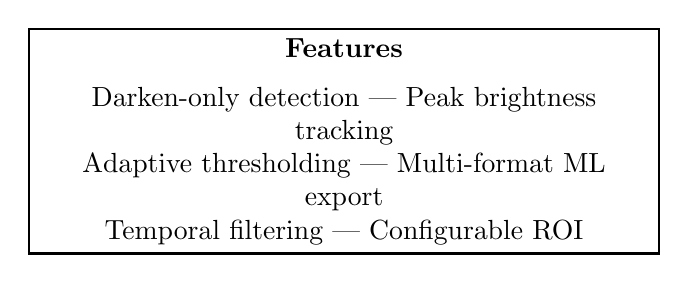
\begin{tikzpicture}
\node[rectangle, draw=black, line width=1pt, minimum width=8cm, minimum height=2cm, fill=white] {
\begin{minipage}{7.5cm}
\centering
\textbf{Features}\\[0.2cm]
Darken-only detection | Peak brightness tracking\\
Adaptive thresholding | Multi-format ML export\\
Temporal filtering | Configurable ROI
\end{minipage}
};
\end{tikzpicture}

\vspace{0.8cm}
\texttt{github.com/j-vaught/vrifa}
\end{center}
\end{frame}

\end{document}
